\documentclass[preview]{standalone}
\usepackage{tkz-graph}
\begin{document}

\begin{figure}[ht]
\center
 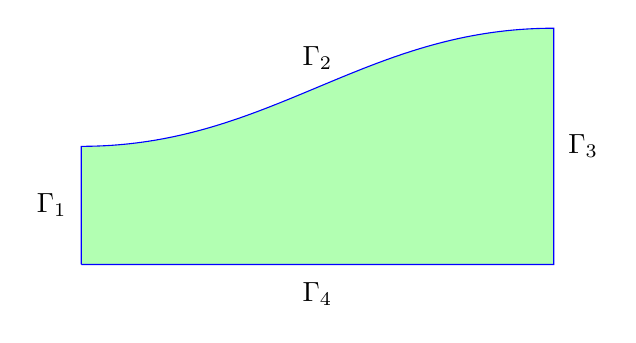
\begin{tikzpicture}[scale=0.75]

   \fill [green!30] (0,0) -- (0,2) to[out=0,in=180] (8,4) -- (8,0) -- (0,0);
   \draw [blue] (0,0) -- (0,2) to[out=0,in=180] (8,4) -- (8,0) -- (0,0);

   \draw(-0.5,1) node {$\Gamma_1$}; 
   \draw(4,3.5) node {$\Gamma_2$}; 
   \draw(8.5,2) node {$\Gamma_3$}; 
   \draw(4,-0.5) node {$\Gamma_4$}; 


 \end{tikzpicture}
\end{figure}





\end{document}



После: convert pdf to png
https://convertio.co/pdf-png/



 






